
\subsection*{Email is not free}

Bureaucracy as distributed knowledge and distributed decision-making requires communication. Because synchronous communication like phone calls, video calls, and in-person meetings is challenging to coordinate, written communication is widely used for asynchronous collaboration. Whether that written content is emails or text-based chat, writing is expensive.

The cost of email includes time spent writing (authorship), time spent reading (readership), and infrastructure costs (e.g., maintenance). Those three factors can be quantified as variables. 
\marginpar{$>>$ Math}%
\begin{multline*}
\text{Cost per email} = 
(\text{hourly rate of writer})*(\text{time spent writing}) +\\
(\text{hourly rate of reader})*(\text{time spent reading})*(\text{number of readers})+\\
\frac{\text{annual salary of maintainer}}{\text{number of emails per year}} + \frac{\text{email server cost}}{\text{number of emails per year}}
\end{multline*}
Plugging in some numbers, suppose an author charging \$50 per hour spends 5 minutes writing an email to 4 people. Each of those four people also charges \$50 per hour and spends 2 minutes on reading. 
\begin{equation*}
50*(5/60) + 50*(2/60)*4 + \frac{100000}{1000000} + \frac{10000}{1000000} = \$10.84
\label{eq:four_readers}
\end{equation*}
The cost to the organization is more than \$10 for one email! The breakdown of the three variables is shown in Figure~\ref{fig:email_pie_chart}. You've probably sent and received more than one email in your professional career as a bureaucrat. 


If the cost of one email doesn't lead you to be careful with communication, consider the cost to the organization of communication. If email consumes 2 hours a day per person (reading and writing), and if staffing is 50\% of the organization's budget, then 
    % (2/8)*0.5
12.5\% of the organization's budget is spent on email. The same math for applies to meetings, so with 2 hours of meeting and 2 hours of email that's 25\% of the organization's personnel budget on coordination.

\begin{figure}
    \centering % 0.7 is too small, as is 0.9
    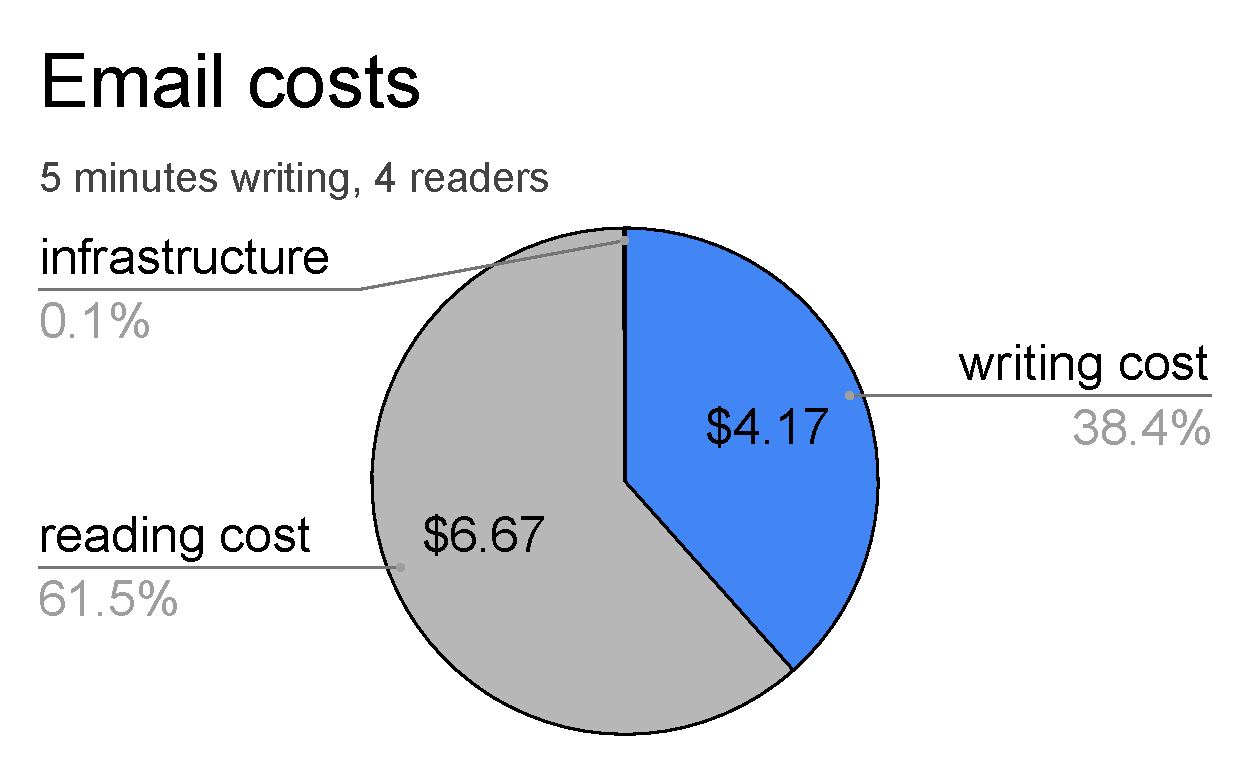
\includegraphics[width=1.1\textwidth]{images/email_costs_5minutes_4people.pdf}
    \caption{Breakdown of costs for one email when the writing took 5 minutes and there were 4 readers. This example assumes an hourly rate of \$50 per person and a reading time of 2 minutes per reader. There are three costs, but infrastructure is too small to see at 0.1\% of the costs.}
    \label{fig:email_pie_chart}
\end{figure}

% https://docs.google.com/spreadsheets/d/1ysV5PA3cEcneKv5BViUhAfgNq26cOlNRj6l5fXuHM3Q/edit?usp=sharing

